\section{Our Solution - Multi-Party Computation (MPC)}\label{sec:scheme}

Our approach to ensure trust in the Sphinx header is to prevent user manipulation by decentralizing the header construction to Trusted Third Parties (TTP) through the use of Multi-Party Computation (MPC).
\newline

We consider TTPs as \textit{honest-but-curious}.
This means that they follow the protocol correctly but may attempt to infer additional information from the data they process.
Our design ensures that TTPs cannot infer any information about the shared secrets \s{i} or the involved mixnodes, even when TTPs collude (except one).
\todo{JT: In the Nym ecosystem, who are the TTPs, who operates them, what exactly are they trusted for?}
\newline

To facilitate explanation and illustration, we describe our solution such that each packet goes through a fixed-length path consisting of three mixnodes.
However, the scheme is general and can be adapted to support arbitrary path lengths. 


\subsection{Header structure}

In our approach, each piece of header information is encoded as an elliptic curve point. 
To achieve this, the encoded string is divided into fixed-size chunks, as illustrated in Figure \ref{fig:chunked_schema}, where each chunk is a single EC point. 
For example, in the case of a path consisting of three mixnodes, the resulting header contains seven EC points: one destination, three mixnodes and three integrity tags.

Therefore a method to encode and decode information to and from elliptic curve points is required. 
Specifically, we require a mapping from integers to curve points, noted \Map{}, and the inverse mapping from curve points to integers, noted \InverseMap{}, 
such that $\InverseMap{\Map{x}} = x$ where $x$ is an integer.

Traditional methods achieve this by directly mapping integers to the x-coordinates of points on the curve. 
However, this approach could leaks information by introducing bias since nearby integers result in nearby points.

To address this, we adopt Elligator, which offers stronger privacy guarantees. 
Unlike the traditional approach, Elligator produces a uniformly distributed output which is computationally indistinguishable from truly random curve points. 
This uniformity is in line with our objectives of preserving anonymity and avoiding linkability. 

\subsection{Protocol description}

The overall decentralized scheme is illustrated in Figure~\ref{fig:overall_schema}.  
The client first computes a sequence of shared secrets and then splits these secrets, along with the IP addresses of the mixnodes in the path and the final destination, into $m$ shares.  
Each set of shares is sent to a different TTP, along with the necessary cryptographic element (\A{}).  
Each TTP independently computes a \textit{partial} Sphinx header using the received shares.  
The client then aggregates these partial headers to reconstruct the final header, ready for transmission through the mixnet.

\begin{figure}[H]
    \centering
    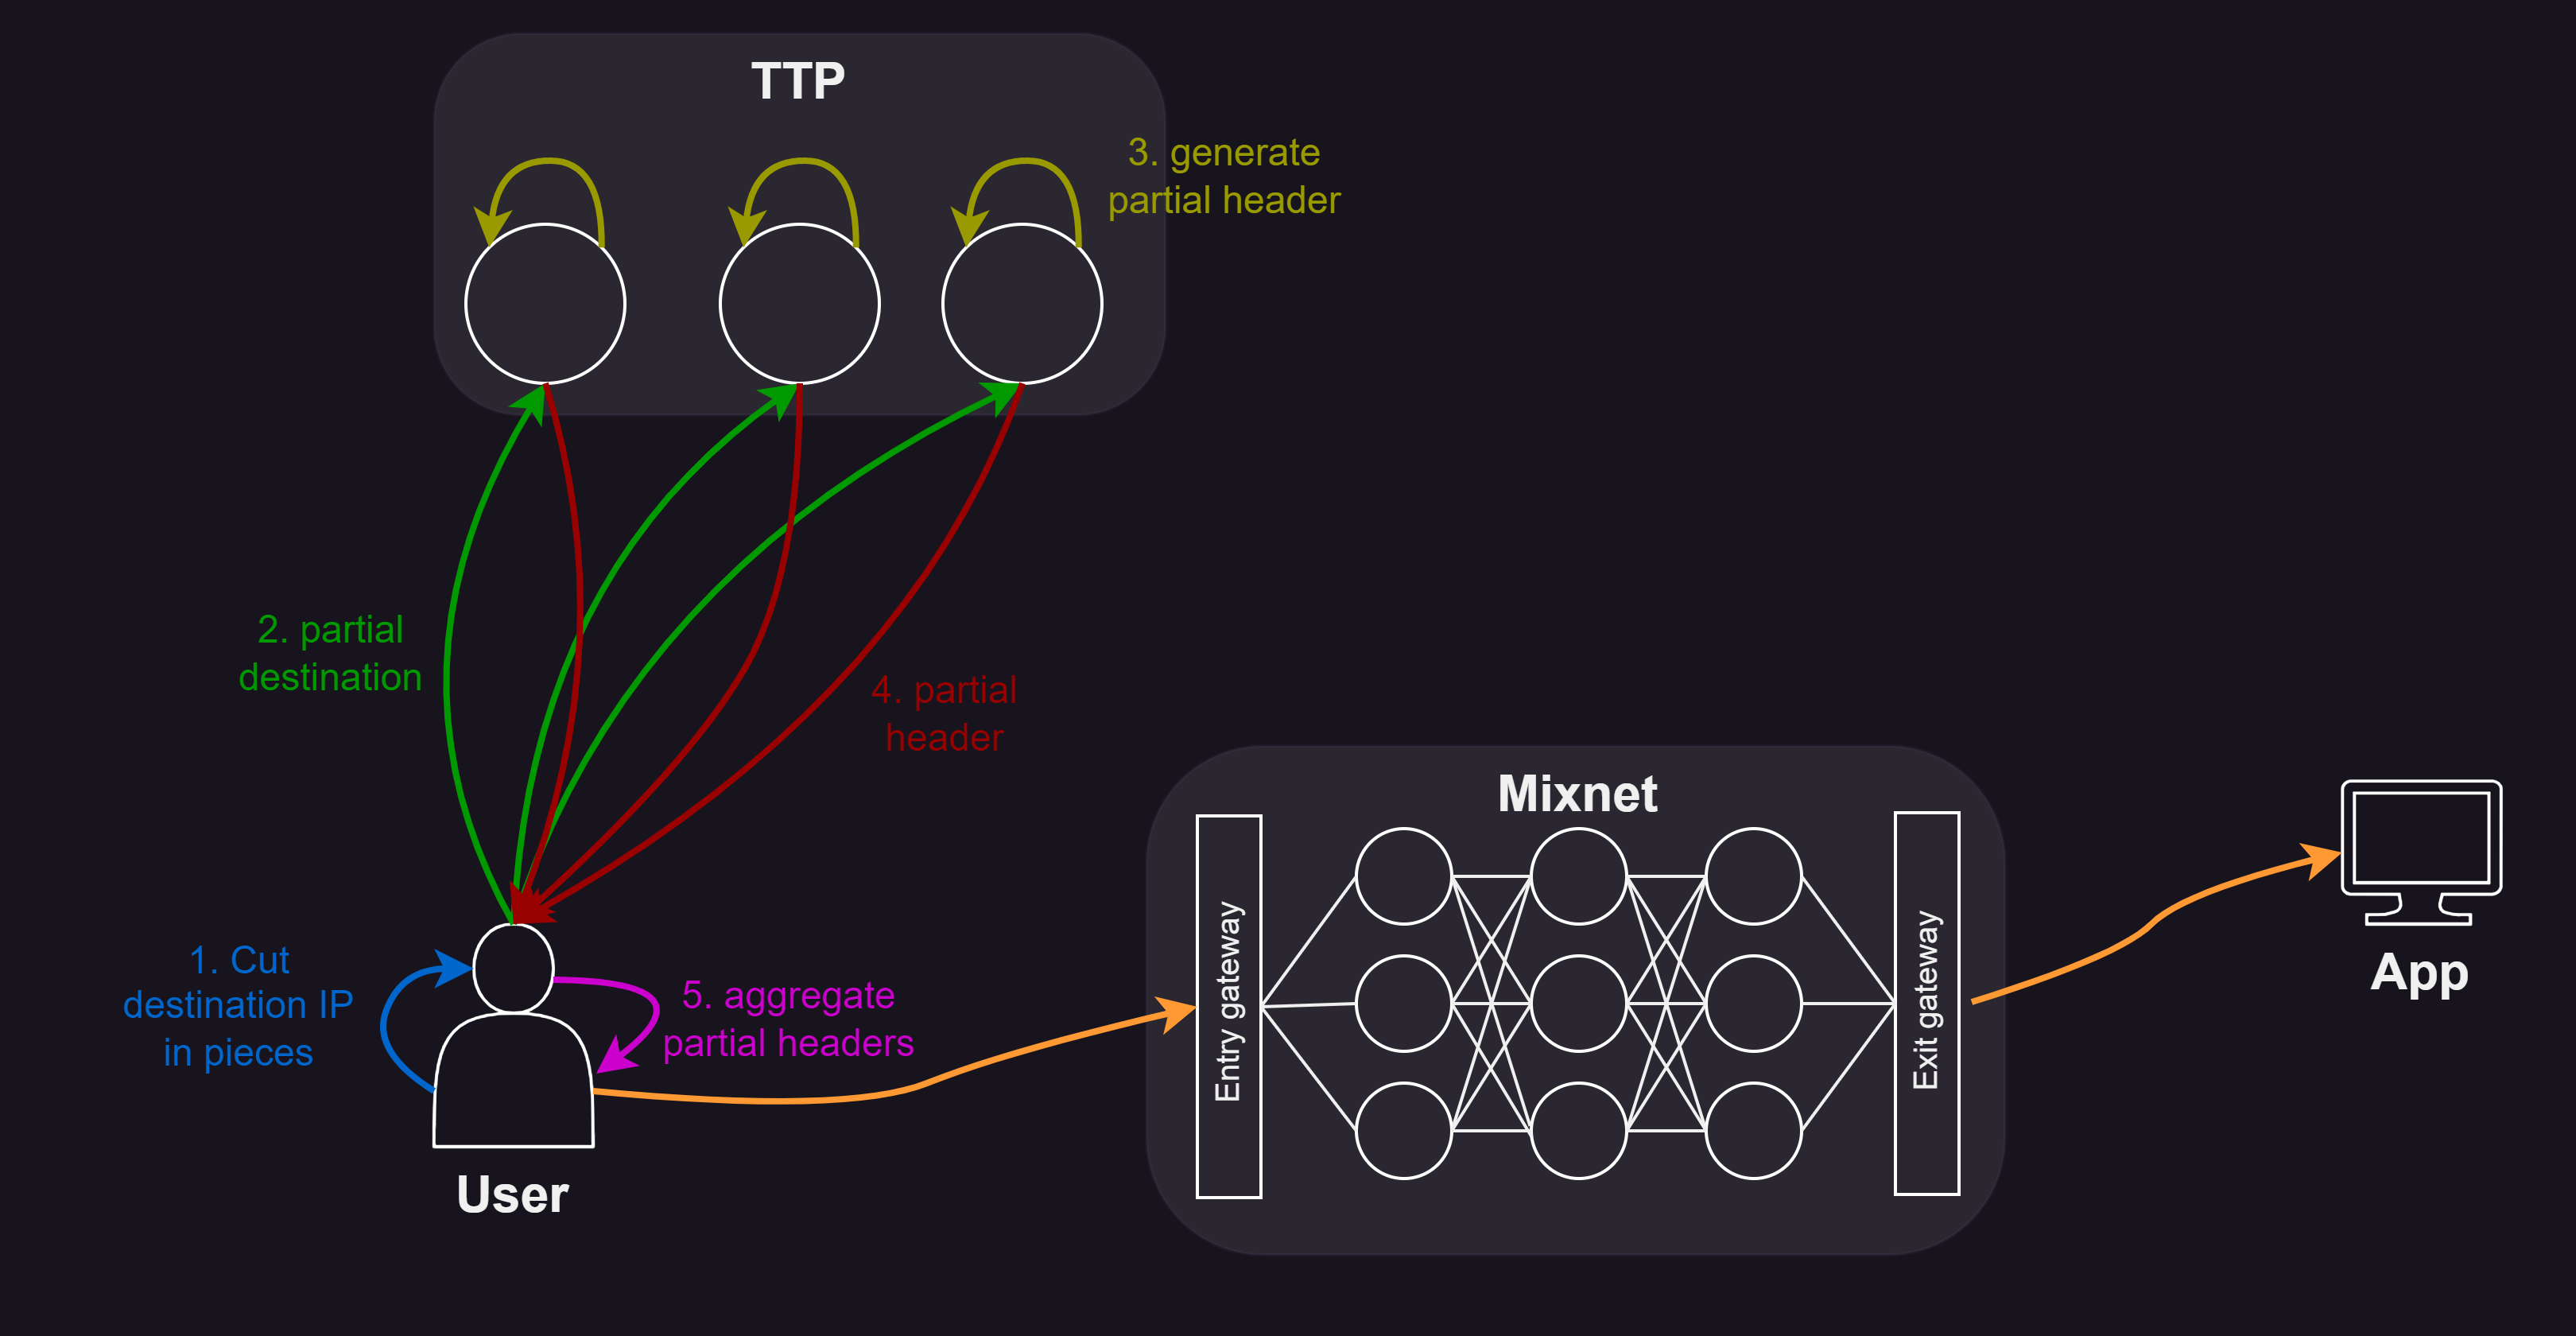
\includegraphics[width=0.8\linewidth]{Images/sphinx_ttp.png}
    \caption{[DRAFT] Overview of the decentralized scheme}
    \label{fig:overall_schema}
\end{figure}\todo{draft image}

\noindent In summary, the protocol is divided into four main steps:
\begin{itemize}
    \item \textbf{Setup}: fixes random points as generators (once but should be refreshed);
    \item \textbf{Client}: splits and shares the necessary information to TTPs;
    \item \textbf{TTP}: encrypts the routing information into a partial header;
    \item \textbf{Mixnode}: decrypts and forwards the header.
\end{itemize}


\subsubsection{Setup}

In our protocol, routing information is divided into seven chunks, each one encoded into an elliptic curve point (see Figure \ref{fig:chunked_schema}). 
These points will later be encrypted by adding a masking point of the form $ P = s G $, where $ s $ is a shared secret and $ G $ is the base generator of the curve.
However, using the same masking point $ P $ for all the seven chunks compromises the \textit{unlinkability} property
(see security note in the TTP step \ref{note:security_why_indep_generators}).

To mitigate this, we use a set of seven \textit{independent} generators $ G_j $, one for each chunk. 
By \textit{independent}, we mean that the scalar relationship between any two generators is unknown. 
Therefore no one knows the scalars $ z_j \in \mathbb{Z}_N $ such that $ G_j = z_j G $.

In principle, this setup phase can be executed only once. 
However, to preserve unlinkability, the set of generators should be refreshed periodically. 
Every entity (clients, mixnodes, and TTPs) must run the setup phase to ensure they use the same set of generators.

To achieve synchronized and deterministic generators across the system, we derive them from a common seed. 
This seed is computed as the hash of the current timestamp, truncated to the chosen refresh interval. 
To produce \textit{independent} generators, we simply increment the seed since Elligator already provides a uniform (i.e. pseudo-random) integers to points mapping.

A subtlety with Elligator is that it can map integers to points outside of the base generator's subgroup.
To ensure that points remain in the generator subgroup, an extra step is required to \textit{clear the cofactor} by multiplying the resulting point by the cofactor (Curve25519's cofactor is $ 8 $).

\noindent The final formula for generating the $ j^{th} $ chunk’s generator is:
\begin{equation}
G_j = 8 \cdot \Map{\hash{\text{timestamp}} + j}, \quad \text{for } j = 1, \dots, 7
\end{equation}


\subsubsection{Client}
% 1) Define a destination
% 2) Select a random path
% 3) Select a random salt $x$ (nonce) 
% 4) Generate a chain of shared secret for the path's mixnode
% 5) Transform IP addresses (path's mixnodes and destination) into Point with Elligator and the split those point into shares.
% 6) Split the shared secrets (int) into shares.
% 7) Send sets of shares (mixnodes IPs, destination IP, shared secrets) to different TTP.
% 8) TTP will compute from those shares a partial header and send it to the client. Afterwards, the client aggregate these partial headers.
  
To send a message to a specific destination, the client first randomly chooses a path through the mixnet and generates a nonce.
Using this nonce and the public keys of each mixnode along the path, the client derives a chain of shared secret integers (\s{1}, \s{2}, \s{3}) as follows:
\begin{equation}
(\s{1}, \s{2}, \s{3}) \quad \left\{ \quad
\begin{aligned}
    \A{i}    &= x_i \, G \\
    \S{i}    &= x_i \, \PK{i} \\
    \s{i}    &= \InverseMap{\S{i}} \\
    r_i      &= \hash{{\A{i}}_y \ \| \ {\S{i}}_y} \\
    x_{i+1}  &= x_i \, r_i \quad (\text{mod}\ n)
\end{aligned}
\right.
\label{eq:shared_secret}
\end{equation}
\todo{Take a look if a schema could be interesting to illustrate Eq. \ref{eq:shared_secret}}
where $ x_1 $ is the client's nonce, $ \PK{i} $ is the public key of the $ i^{th} $ mixnode in the path ($\PK{i} = \sk{i}\G{}$), 
$ n $ is the subgroup order (i.e. $(n+1)\G{} = \G{}$), $ \| $ is  the concatenation operator and subscript $ y $ refers to the $ y $-coordinate of the point.
The scalar $ r_i $ acts as a pseudo-randomizer to update the secret $ x_i $ for the next hop, 
ensuring that each cryptographic element $ \A{i} $ remains unlinkable across mixnodes.

The IP addresses of the mixnodes and the destination are padded with random bits
then mapped to elliptic curve points using Elligator, allowing later recovery of these addresses.
Both the resulting IP points and the shared secrets are split into shares and distributed to $ m $ different TTPs. 
In addition, the client send the hash of each shared secret to these TTPs. % for integrity

Each TTP then independently computes a partial header from the received shares and returns it to the client. 
The client aggregates these partial headers by performing chunk-wise point additions to reconstruct the complete encrypted header.
Finally, the client sends the header along with \A{1} to the first mixnode from the path. 

\subsubsection{TTP}
% 1) Receive partial destination, path's nodes and partial shared secret
% 2) First
% 3) For each layer
Each TTP receives from the client:
\begin{itemize}
    \item a share of the destination address (EC point noted $ \Delta $);
    \item a share of each mixnode address in the path (EC points noted $ \N{i} $);
    \item a share of each shared secrets (integers noted $ \s{i} $);
    \item the hash of each shared secrets (integers noted $ \sHashed{i} $).
\end{itemize}

The TTP constructs a partial encrypted header by layering routing information in reverse path order, starting from the last mixnode, as illustrated by Figure \ref{fig:chunked_schema}.

At each layer, two new chunks are introduced: the next mixnode’s \todo[color=purple!30]{what is the best formulation: "next mixnode" or "mixnode from previous layer" ?} address (\N{i+1}) and the integrity tag (\C{i+1}).  
To preserve a fixed-length header while allowing mixnodes to reverse the operation (as in the original design), four additional \emph{filler chunks} are appended.  
These filler chunks are carefully computed such that at each layer, after applying the corresponding masking points (\sG{i}{j}\hspace{-1mm}), the last two chunks cancel out and become identity point (i.e. point at infinity).  
This mechanism allows these two chunks to be safely truncated at each layer, ensuring a consistent header size while preserving reversibility for mixnodes.

To initialize the header, the TTP encrypts the destination point using the shared secret of the last mixnode and append the required filler chunks. 
Let $ \Delta $ be the partial destination point, \s{i} the partial shared secret corresponding to the $ i^\text{th} $ mixnode in the path, and $ G_j $ the $ j^\text{th} $ chunk's generator. 
The chunks for the last layer (assuming a 3-hop path) are computed as follows:
\begin{equation}
\B{3}{} \quad \left\{ \quad
\begin{aligned}
    \B{3}{1} &= \Delta       + \sG{3}{1} \\
    \B{3}{2} &= - (\sG{2}{4} + \sG{1}{6}) \\
    \B{3}{3} &= - (\sG{2}{5} + \sG{1}{7}) \\
    \B{3}{4} &= - \sG{2}{6} \\
    \B{3}{5} &= - \sG{2}{7} \\
\end{aligned}
\right.
\label{eq:last_layer}
\end{equation}

\noindent
Subsequent layers ($ i = 2 $ and $ i = 1 $) are computed with Eq. \ref{eq:layer_i} where \N{i+1} represents the 
elliptic curve point corresponding to the $ (i+1)^\text{th} $ mixnode in the path and \C{i+1} is the integrity tag from previous layer.
\begin{equation}
\B{i}{} \quad \left\{ \quad
\begin{aligned}
    \B{i}{1} &= \N{i+1} + \sG{i}{1}\\
    \B{i}{2} &= \C{i+1} + \sG{i}{2} \\
    \B{i}{3} &= \B{i+1}{1} + \sG{i}{3} \\
    \B{i}{4} &= \B{i+1}{2} + \sG{i}{4} \\
    \B{i}{5} &= \B{i+1}{3} + \sG{i}{5} \\
\end{aligned}
\right.
\label{eq:layer_i}
\end{equation}
\todo[color=purple!30]{$\B{i+1}{1}$ is a light notation for $\B{(i+1,}{1)}$, should I put the full notation for clarity ?}

\noindent
For each layer, the integrity tag is computed with Eq. \ref{eq:integrity} where \hashIt{\sHashed{i}}{j} means hashing $j$ times \sHashed{i} which is the hash of the $i^{th}$ mixnode's complete shared secret.
The integrity tag consists in a pseudo-random weighted sum of the chunks, offset by a secret point derived from the shared secret integer.
The pseudo-random weights (i.e. \hashIt{\sHashed{i}}{j-1}) ensure binding, preventing adversaries from modifying individual chunks.
Without these weights, an attacker could add a random point P to one chunk and subtract P from another, thereby preserving the overall sum and bypassing the integrity check.
The secret offset (i.e. \sG{i}{}) prevents curious TTPs from correlating integrity tags.
Since TTPs are aware of these pseudo-random weights, omitting this offset would allow them to potentially link some incoming and outgoing mixnode's packets by simply verifying integrity tags.
\begin{equation}
\C{i} = \sG{i}{} + \sum_{j=1}^{5} \big( \hashIt{\sHashed{i}}{j-1} \, \B{i}{j} \big)
\label{eq:integrity}
\end{equation}

When the first layer is finally computed, it is appended with the integrity tag \C{1} and the first mixnode’s point $ N_1 $.
Finally, the TTP returns the constructed partial header to the client.

\begin{figure}[H]
    \centering
    \resizebox{0.9\linewidth}{!}{
\centering
\begin{tikzpicture}
    % \tiny
    \setlength{\y}{0cm}

    \node (ip) [block=1] at (0, \y) {$\mathrm{\Delta}$};
    \vgap
    \node (s3_) [block=7] at (0, \y) {};
    \node [inblock=1] at (0, \y) {\sG{3}{1}};
    \foreach \j in {1,...,6} {
        \node [inblock=1, gray] at (\j*\width, \y) {}; 
    }
    \vgap
    \node (s2_) [block=7] at (- 2*\width, \y) {};
    \foreach \j in {0,...,2} {
        \node [inblock=1, gray] at (-\j*\width, \y) {}; 
    } 
    \foreach \j in {4,...,7} {
        \node [inblock=1] at (\j*\width - 3*\width, \y) {\sG{2}{\j}}; 
    }
    \vgap
    \node (s1_) [block=7] at (- 2*\width, \y) {};
    \foreach \j in {0,...,2} {
        \node [inblock=1, gray] at (-\j*\width, \y) {}; 
    }
    \foreach \j in {4,...,5} {
        \node [inblock=1] at (\j*\width - 3*\width, \y) {\sG{1}{\j}}; 
    }
    \foreach \j in {3,...,4} {
        \node [inblock=1, gray] at (\j*\width, \y) {}; 
    }
    \vgap 
    \foreach \j in {1,...,5} {
        \node (B3\j) [inblock=1] at (\j*\width-\width, \y) {\B{3}{\j}}; 
    }
    \node (xor3) [] at (-3*\width, \y) {\normalsize $ + $}; 
    \vGap
    \node (hmac3) [HMAC, fill=white] at (1.5*\width, \y) {\hmac};
    \vGap

    \node (n3) [block=1] at (0, \y) {\N{3}}; 
    \node (y3) [block=1] at (\width, \y) {\C{3}}; 
    \foreach \j in {1,...,5} {
        \node (b3\j) [inblock=1] at (\width + \j*\width, \y) {\B{3}{\j}}; 
    }
    \vgap
    \foreach \j in {1,...,7} {
        \node (s2\j) [inblock=1] at (\j*\width-\width, \y) {\sG{2}{\j}};
    }
    \vgap
    \foreach \j in {1,...,5} {
        \node (B2\j) [inblock=1] at (\j*\width-\width, \y) {\B{2}{\j}}; 
    }
    \node (zero2) [zero_pad=2] at (5*\width, \y) {0}; 

    \node (xor2) [] at (-\width, \y) {\normalsize $ + $}; 
    \vGap
    \node (hmac2) [HMAC, fill=white] at (1.5*\width, \y) {\hmac};
    \vGap

    \node (n2) [block=1] at (0, \y) {\N{2}}; 
    \node (y2) [block=1] at (\width, \y) {\C{2}}; 
    \foreach \j in {1,...,5} {
        \node (b2\j) [inblock=1] at (\width + \j*\width, \y) {\B{2}{\j}}; 
    }
    \vgap
    \foreach \j in {1,...,7} {
        \node (s1\j) [inblock=1] at (\j*\width-\width, \y) {\sG{1}{\j}};
    }    
    \vgap
    \foreach \j in {1,...,5} {
        \node (B1\j) [inblock=1] at (\j*\width-\width, \y) {\B{1}{\j}};
    }
    \node (zero1) [zero_pad=2]  at (5*\width, \y) {0}; 

    \node (xor1) []  at (-\width, \y) {\normalsize $ + $ }; 
    \vGap
    \node (hmac1) [HMAC, fill=white]  at (1.5*\width, \y) {\hmac};
    \vGap

    \node (n1) [block=1]  at (0, \y) {\N{1}}; 
    \node (y1) [block=1]  at (\width, \y) {\C{1}};
    \foreach \j in {1,...,5} {
        \node (b1\j) [inblock=1]  at (\width + \j*\width, \y) {\B{1}{\j}}; 
    }

    %% XOR ARROWS %%
    % 3
    \draw[arrow] (ip.west) -- ++(-3*\width, 0) -- (xor3.north);
    \draw[arrow] (s3_.west) -- ++(-3*\width, 0) -- (xor3.north);
    \draw[arrow] (s2_.west) -- ++(-\width, 0) -- (xor3.north);
    \draw[arrow] (s1_.west) -- ++(-\width, 0) -- (xor3.north);
    \draw[arrow] (xor3.east) -- (B31.west);
    % 2
    \draw[arrow] (n3.west) -- ++(-\width, 0) -- (xor2.north);
    \draw[arrow] (s21.west) -- ++(-\width, 0) -- (xor2.north);
    \draw[arrow] (xor2.east) -- (B21.west);
    % 1
    \draw[arrow] (n2.west) -- ++(-\width, 0) -- (xor1.north);
    \draw[arrow] (s11.west) -- ++(-\width, 0) -- (xor1.north);
    \draw[arrow] (xor1.east) -- (B11.west);

    %% HMAC ARROWS %%
    % 3
    \node[left=\width of hmac3] (input_hmac3) {\sG{3}{}};
    \draw[arrow] (input_hmac3) -- (hmac3.west);
    \draw [decorate, decoration={brace, amplitude=3pt, mirror, aspect=0.3, raise=2pt}] (B31.south west) -- (B35.south east);
    
    \draw[arrow] (hmac3.south) -- (y3.north);
    % 2
    \node[left=\width of hmac2] (input_hmac2) {\sG{2}{}};
    \draw[arrow] (input_hmac2) -- (hmac2.west);
    \draw [decorate, decoration={brace, amplitude=3pt, mirror, aspect=0.3, raise=2pt}] (B21.south west) -- (B25.south east);
    \draw[arrow] (hmac2.south) -- (y2.north);
    % 1
    \node[left=\width of hmac1] (input_hmac1) {\sG{1}{}};
    \draw[arrow] (input_hmac1) -- (hmac1.west);
    \draw [decorate, decoration={brace, amplitude=3pt, mirror, aspect=0.3, raise=2pt}] (B11.south west) -- (B15.south east);
    \draw[arrow] (hmac1.south) -- (y1.north);

    %% BETA ARROWS %%
    \begin{pgfonlayer}{background}
        % 3
        \foreach \j in {1,...,5} {
            \draw[->, dashed, very thin, color=lightgray] (B3\j.south) -- ([xshift=-1pt, yshift=+1pt] b3\j.north);
        }
        % 2
        \foreach \j in {1,...,5} {
            \draw[->, dashed, very thin, color=lightgray] (B2\j.south) -- ([xshift=-1pt, yshift=+1pt] b2\j.north);
        }
        % 1
        \foreach \j in {1,...,5} {
            \draw[->, dashed, very thin, color=lightgray] (B1\j.south) -- ([xshift=-1pt, yshift=+1pt] b1\j.north);
        }
    \end{pgfonlayer}

    %% TEST ANNOTATION %%
    \color{lightgray}
    \draw [decorate, very thin, decoration={brace, amplitude=3pt, raise=2*\width+30pt}]
        ([xshift=4*\width] ip.north east) -- (B35.south east) node[midway, xshift=110pt]{Eq. \ref{eq:last_layer}};
    \draw [decorate, very thin, decoration={brace, amplitude=3pt, raise=30pt}]
            (b35.north east) -- (zero2.south east) node[midway, xshift=70pt]{Eq. \ref{eq:layer_i} ($i=2$)};
    \draw [decorate, very thin, decoration={brace, amplitude=3pt, raise=30pt}]
            (b25.north east) -- (zero1.south east) node[midway, xshift=70pt]{Eq. \ref{eq:layer_i} ($i=1$)};
    % \draw [decorate, very thin, decoration={brace, amplitude=3pt, raise=10pt}]
    %         ([xshift=2*\width, yshift=-2pt] B35.south east) -- ([yshift=2pt] b35.north east) node[midway, xshift=30pt]{Eq. \ref{eq:integrity}};
    % \draw [decorate, very thin, decoration={brace, amplitude=3pt, raise=10pt}]
    %         ([xshift=2*\width, yshift=-2pt] B25.south east) -- ([yshift=2pt] b25.north east) node[midway, xshift=30pt]{Eq. \ref{eq:integrity}};
    % \draw [decorate, very thin, decoration={brace, amplitude=3pt, raise=10pt}]
    %         ([xshift=2*\width, yshift=-2pt] B15.south east) -- ([yshift=2pt] b15.north east) node[midway, xshift=30pt]{Eq. \ref{eq:integrity}};
    \node[right=6*\width+10pt of hmac3] {Eq. \ref{eq:integrity}};
    \node[right=6*\width+10pt of hmac2] {Eq. \ref{eq:integrity}};
    \node[right=6*\width+10pt of hmac1] {Eq. \ref{eq:integrity}};
\end{tikzpicture}}
    \caption{Chunk-wise header encryption (TTP side), where \eq[x] refers to Eq. x.}
    \label{fig:chunked_schema}
\end{figure}


\paragraph{\textbf{Security Note.}}\label{note:security_why_indep_generators}
To preserve unlinkability, it is essential that the generators $ (\G{1}, \dots, \G{7}) $ are \textit{independent}, meaning that their scalar relationships are unknown and cannot be derived.
If the same generator \G{} were used across chunks (or their scalar relationships known), an adversary could compute the chunk-wise difference between consecutive layers: $ \B{i}{j} - \B{i+1}{j} = \sG{i}{} $.
Since the shared secret \s{i} remains consistent within a layer, the resulting differences would reveal a predictable pattern (uniform or preserved scalar relationships).
This consistency could allow an adversary to correlate incoming and outgoing packets at a mixnode, thereby breaking the unlinkability property.
Using independent generators for each chunk prevents such correlations and is therefore critical to the protocol's security.  


\subsubsection{Mixnode}
% 1) Extract information from the header
% 2) Recompute shared secret
% 3) Integrity check
% 4) Update encrypted information (β)
% 5) Update cryptographic element (α)

When a packet arrives at mixnode $i$, it begins by extracting the relevant header fields, namely the cryptographic element \A{i} and the integrity tag \C{i}.  
The mixnode then recomputes the shared secret point \S{i} using its private key \sk{i} and the cryptographic element \A{i}:  
\begin{equation}
\begin{aligned}
    \S{i} &= \sk{i} \, \A{i} \\
    \s{i} &= \InverseMap{\S{i}}\\
\end{aligned}
\label{eq:derive_secret}
\end{equation}
This shared secret point is subsequently mapped to the shared integer \s{i} using Elligator inverse mapping.
This shared integer is then used to verify the integrity tag (Eq. \ref{eq:integrity_check}).
\begin{equation}
\C{i} \overset{\text{?}}{=} \sG{i}{} + \sum_{j=1}^{5} \big( \hashIt{\s{i}}{j} \, \B{i}{j} \big)
\label{eq:integrity_check}
\end{equation}

\noindent If the integrity check passes, the mixnode pads the header by appending two \textit{identity} chunks (i.e. point at infinity) and then updates it as:
\begin{equation}
{\BB{i}{j}} = \B{i}{j} - \sG{i}{j} \qquad \forall j = 1, \dots, 7
\label{eq:decrypt}
\end{equation}

The first chunk ({\BB{i}{1}}), encodes the next mixnode’s IP address (\N{i+1}). 
This point is mapped back to an integer using Elligator and the random padding is removed by keeping the last 128 bits (i.e. size of an IP address).

\noindent The second chunk ({\BB{i}{2}}) is the next integrity tag (\C{i+1}) for the remaining five chunks that form the new encrypted routing information (\B{i+1}{}).

To maintain unlinkability, the cryptographic element \A{i} must be updated for the next hop. 
As in the client's step, it is computed using the $y$-coordinates of both \A{i} and \S{i}:
\begin{equation}
\A{i+1} = \text{hash}({\A{i}}_y \ \| \ {\S{i}}_y) \ \A{i}
\label{eq:update_alpha}
\end{equation}
Finally, the mixnode forwards the updated header (\A{i+1}, \C{i+1}, \B{i+1}{}) to the next node.

\begin{figure}[H]
    \centering
    \resizebox{0.9\linewidth}{!}{\centering
\begin{tikzpicture}
    %% INPUT
    \node (L0) at (0,0) {};
    \node (A) [block=1] at (L0) {\A{i}};
    \node (B) [block=5] at ($(A.east) + (\width, 0)$)  {\B{i}{}};
    \node (C) [block=1] at ($(B.east) + (2*\width, 0)$) {\C{i}};

    %% LINE 1 (shared secret, check integrity & decrypt)
    \node (L1) at ($(L0) - (0, 2.5*\height)$) {};
    \node (sk) [block=1] at ($(L1) - (2*\width, 0)$) {$sk_i$};
    \node (ss) [op] at ($(A |- L1) - (0.25*\width, 0)$) {\ref{eq:derive_secret}};
    \node (S) [block=1] at (A.east |- L1)  {$S$};
    \node (check) [op] at ($(C |- L1) + (0, 2pt)$)  {\ref{eq:integrity_check}};
 
    %% LINE 2 (decryption & blind)
    \node (L2) at ($(L1) - (0, 2.1*\height)$) {};
    \foreach \j in {1,...,5} {
        \node (B\j) [inblock=1, xshift=\j*\width] at ($(B.west |- L2) - (\width, 0)$) {\B{i}{\j}};
    }
    \node (pad) [zero_pad=2] at (B5.east) {0}; 
    \foreach \j in {1,...,7} {
        \node (sG\j) [inblock=1, xshift=\j*\width] at ($(B1.west) - (\width, 1.2*\height)$) {\sG{}{\j}};
    } 
    \node (N'_) [block=1] at ($(sG1.west) - (0, 2*\height)$) {\N{i+1}};
    \node (C'_) [block=1] at (N'_.east) {\C{i+1}};
    \node (B'_) [block=5] at (C'_.east)  {\B{i+1}{}};
    \node (xor) [op] at ($(check |- sG1) - (0, \height)$) {\ref{eq:decrypt}};
    \node (blind) [op] at ($(A |- xor) + (0.25*\width, 0)$) {\ref{eq:update_alpha}};
    
    %% BOX
    \node (mixnode) [draw=red, dashed, fit=(sk) (B'_) (check)] {};
    \node[xshift=4pt, yshift=10pt] at (sk.north) {\color{red} \textbf{Mixnode $i$}};

    %% OUTPUT
    \node (L) at ($(mixnode.south) - (0, 2.5*\height)$) {};
    \node[] (N') at (sk |- L.north) {Next};
    \node[yshift=-7pt] at (sk |- L.north) {mixnode};
    \node (A') [block=1] at (A.west |- L) {\A{i+1}};
    \node (B') [block=5] at (B.west |- L)  {\B{i+1}{}};
    \node (C') [block=1] at (C.west |- L) {\C{i+1}};

    %% ARROW
    % (6) shared secret
    \draw[arrow] (A.south -| ss) -- (ss);
    \draw[arrow] (sk) -- (ss);
    \draw[arrow] (ss) -- (S);
    % (7) check
    \draw[arrow] (B.south) |- (check.+153);
    \draw[arrow] (C) -- (check);
    \draw[arrow] (S.east |- check.-153) -- (check.-153);
    % (8) xor
    \draw[arrow] (pad) -| (xor);
    \draw[arrow] (sG7) -| (xor);
    \draw[arrow] (xor) |- (B'_);
    % (9) blind
    \draw[arrow] (A.south -| blind) -- (blind);
    \draw[arrow] (S) |- (blind);
    \draw[arrow] (blind) -- (blind |- A'.north);
    % xor block
    \draw[arrow] (B) -- (B.south |- B1.north);
    \draw[arrow] (S) |- (sG1);
    % output
    \node (tmp) at ($(mixnode.south) - (0, 0.5*\height)$) {};
    \draw[arrow] (N'_) -- (N'_ |- tmp) -| (N');
    \draw[arrow] (C'_) -- (C'_ |- tmp) -| (C');
    \draw[arrow] (B'_) -- ($(B'_ |- tmp) - (0, 7pt)$) -| (B');

\end{tikzpicture}}
    \caption{Processing sphinx header at mixnode $i$, where \eq[x] refers to Eq. x.}
    \label{fig:mixnode_decryption}
\end{figure}
